%----------------------------------------------------------------------------------------
%	SECTION 1.1
%----------------------------------------------------------------------------------------

\section{Discrete Random Variables.}
\label{section1}

\begin{definition}
    Let $X$ be a discrete random variable with finite, or countable range $R$,
    $R=\{x_1, x_2, \dots\}$. Let $p_i=P(X=x_i)$. We define the \textbf{entropy}
    base $b$ of  $X$ to be:
    \begin{equation}
        H_b(X)=\sum_{i \geq 1}{p_i\log_b{\inv{p_i}}}
    \end{equation}
    If $b=2$, we write $\log_2=\log$ and if  $b=e$ we write  $\log_e=\ln$.
    Additionally, we define  $p_i\log_b{\inv{p_i}}=0$ whenever $p_i=0$. We
    define  $H(X)=\infty$ in the case that $R$ is infinite and  $H$ diverges.
\end{definition}

\begin{example}
    \begin{enumerate}
        \item[(1)] If $X$ is the outcome of the roll of a fair $6$-sided die,
        then $R=\{1,2,3,4,5,6\}$ and $p_i=\frac{1}{6}$. Thus,
        $H_b(X)=\log_b{6}$.

    \item[(2)] Let $R=\faktor{\Z}{2\Z}$, and define $X$ by the prbabilities
        $P(X=0)=p$ and $P(X=1)=1-p$. Then $H_2(X)=-p\log{p}-(1-p)\log{(1-p)}$.
        We call $H_2$ the \textbf{binary entropy function} and denote it simply
        as $H$. The majority of the work done in these notes will concern this
        function in particular.

        \begin{figure}
            \centering
            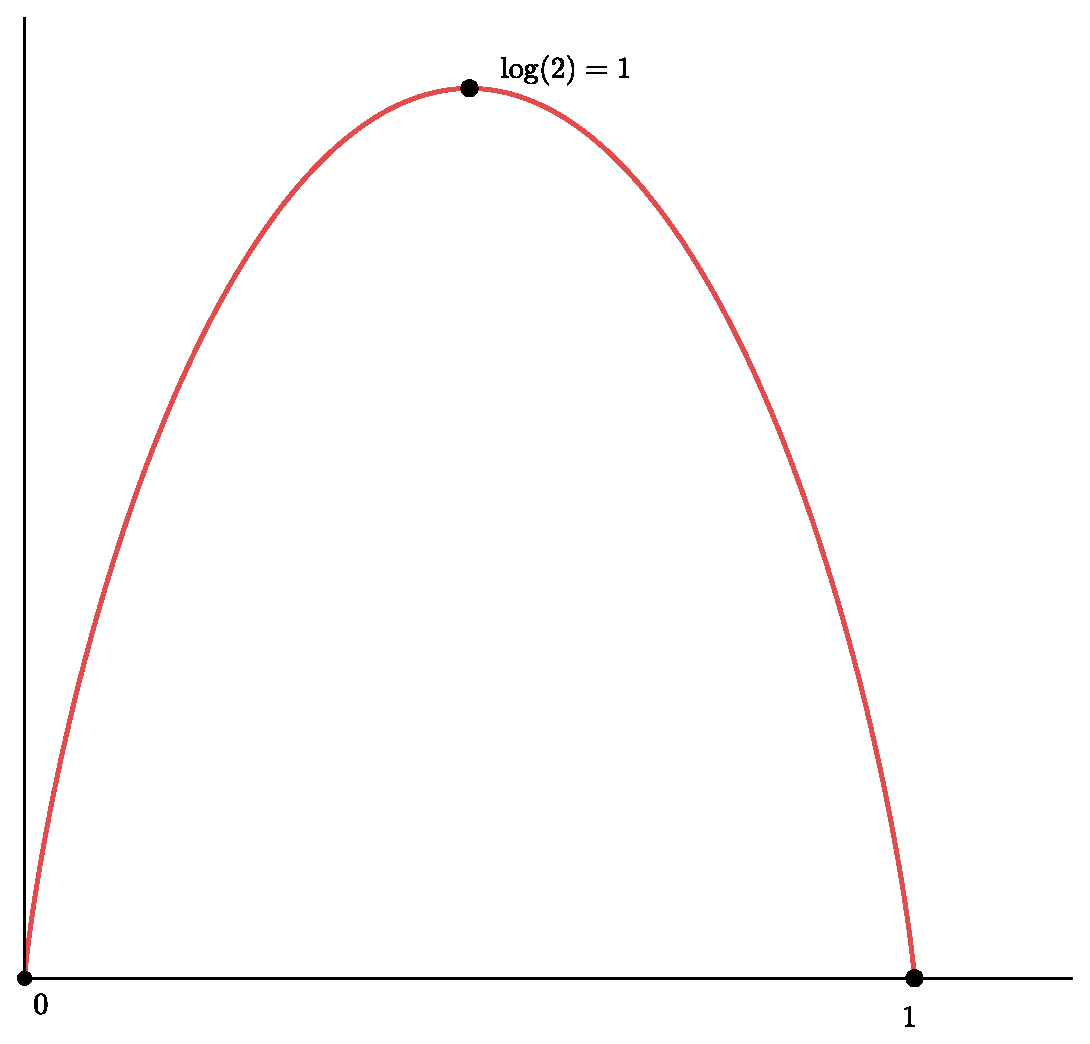
\includegraphics[scale=0.3]{Figures/Chapter2/binary_entropy.eps}
            \caption{The graph of the binary entropy function $H_2(X)=H(X)$.
            Notice that $H(X)=0$ at $0$ and  $1$.}
            \label{fig_2.1}
        \end{figure}

    \item[(3)] If $p=(p_1, \dots, p_r)$ is any probability vector (where $p_i
        \geq 0$ and  $\sum{p_i}=1$), we define the \textbf{entropy function}
        base $b$ of  $p$ to be  $H(p)=H(p_1, \dots,
        p_r)=\sum{p_i\log{\inv{p_i}}}$.

    \item[(4)] If $A=\sum_{n=2}^{\infty}{\inv{n\log^2{n}}}$, and if $X$ is a
        random variable defined by  $P(X=n)=\inv{An\log^2{n}}$, for $n \geq 2$,
        then  $H(X)=\infty$.
    \end{enumerate}
\end{example}

\begin{definition}
    Let $X$ be a discrete random variable with range  $R$. We define the
    \textbf{ammount of information} in base $b$, provided by the event $X=x$ to
    be the function $I_b(x)=-\log_b{P(X=x)}$, where $x \in R$. When $b=2$, we
    write  $I_b=I$.
\end{definition}

\begin{lemma}\label{2.1.1}
    For any discrete random variable $X$, $H_b(X)=E(I_b(X))$.
\end{lemma}
\begin{proof}
    This follows from the definitions of $I_b(X)$, $H_b(X)$, and the expectation
    $E(I_b(X))$.
\end{proof}

\begin{example}
    Define $X$ by the probabilities  $P(X=0)=P(X=1)=\frac{1}{2}$. Then
    $I(0)=I(1)=H(X)=\log{2}$.
\end{example}

\begin{theorem}\label{2.1.2}
    Let $X$ be a discrete random variable with range  $R=\{x_1, \dots, x_r\}$.
    Then:
    \begin{equation}
        0 \leq H_b(X) \leq \log{r}
    \end{equation}
    Furthermore, $H_b(X)=0$ if, and only if $p_i=1$ for some  $i$, and
    $H_b(X)=\log{r}$ if, and only if $p_i=\frac{1}{r}$ for all $i$.
\end{theorem}
\begin{proof}
    Since each $0 \leq p_i \leq 1$, $\inv{p_i} \geq 0$, thus $\log{\inv{p_i}}
    \geq 0$. This implies that $H_b(X) \geq 0$. Now, $p\log{\inv{p}}=0$ if, and
    only if $p=0$ or  $p=1$. Thus,  $H_b(X)=0$ if and only if $p=0$ or  $p=1$,
    that is, if each $p_i=0$ or each  $p_i=1$.

    Notice now, that the function  $\log{x}$ is convex down. Thus, by theorem
    \ref{1.2.5}, we get $H(X)=\sum{p_i\log{\inv{p_i}}} \leq
    \sum{p_i\frac{1}{p_i}}=\log{r}$, so $H_b(X)=\log{r}$ if, and only if $p_i$
    is constant for each  $i$, i.e.  $p_i=\frac{1}{r}$ for all $i$.
\end{proof}
\begin{corollary}
    If $p=(p_1, \dots, p_r)$ is a probability vector, then $H_b(P)$ attains its
    maximum value at uniquely $p=(\frac{1}{r}, \dots, \frac{1}{r})$.
\end{corollary}

\begin{definition}
    Let $X$ and  $Y$ be random variables. We define the  \textbf{conditional
    entropy} of $X$ given  $Y$ to be the entropy  $H(X|Y)$ defined by:
    \begin{equation}
        H(X|Y)=E(\log{\inv{p(x|y)}})
    \end{equation}
    Where $P(X|Y)=P(X=x, Y=y)$. We again define $0\log{0}=0$ and $H(X|Y)=\infty$
    whenever the expectation diverges.
\end{definition}
\begin{remark}
    The notion of conditional entropy can also be motivated by a model of a
    communications channel called the \textbf{discrete memoryless channel}
    (DMC). DMC accept a $r$ input symbols and  give $s$ output symbols. The
    channel is memoryless as the current output only depends on the current
    input and not any previous inputs. DMCs can be visualized in the following
    figures \ref{fig_2.2} and \ref{fig_2.3}. We can describe the behaviour of a
    DCM with an $r \times s$ matrix of  \textbf{transition proabilities},
    $(p(x|y))$, where the $ij$-th entry is the probability  $p(i|j)$.
\end{remark}

\begin{figure}[h]
    \centering
    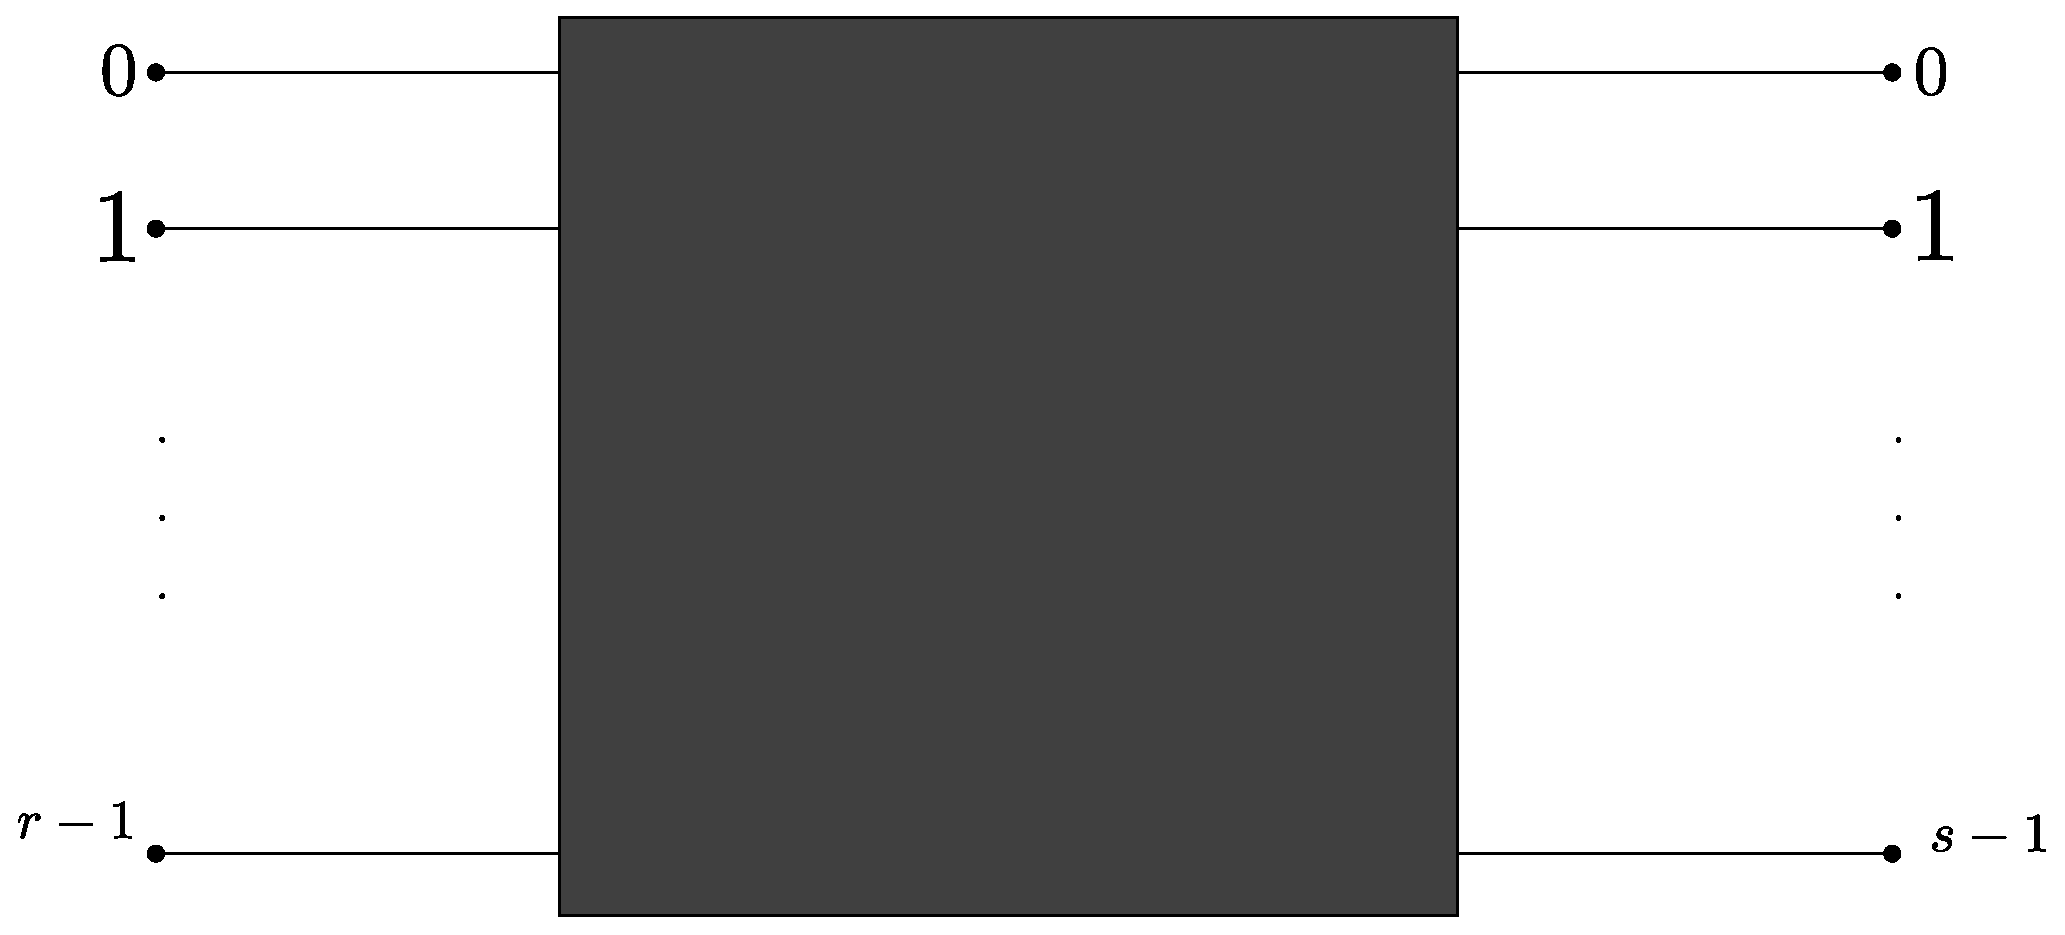
\includegraphics[scale=0.3]{Figures/Chapter2/dmc_1.eps}
    \caption{A discrete memoryless channel viewed as a black box.}
    \label{fig_2.2}
\end{figure}

\begin{figure}[h]
    \centering
    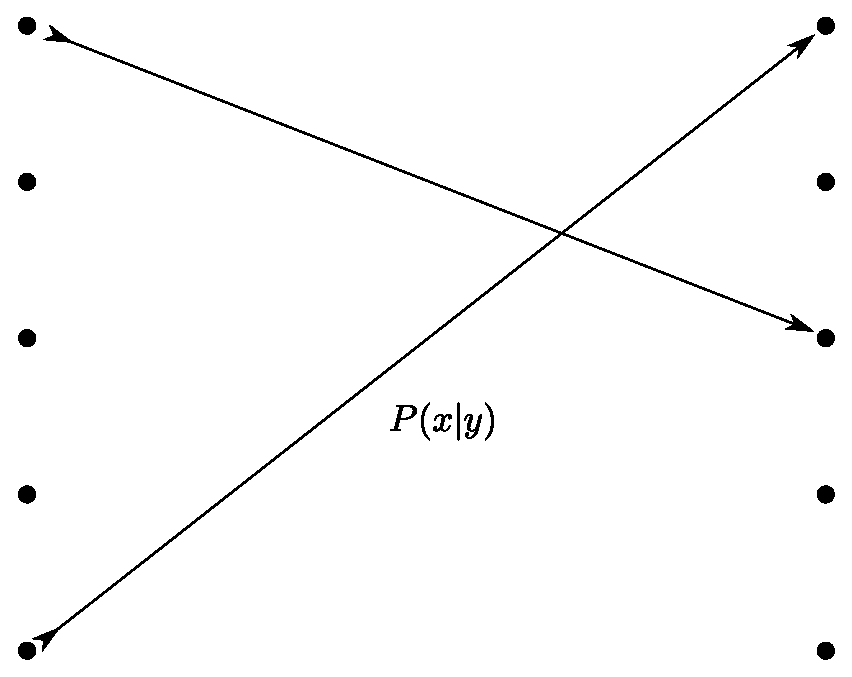
\includegraphics[scale=0.3]{Figures/Chapter2/dmc_2.eps}
    \caption{A discrete memoryless channel viewd in terms of the current inputs
    and outputs.}
    \label{fig_2.3}
\end{figure}

\begin{example}
    \begin{enumerate}
        \item[(1)] We define a \textbf{binary symmetric source} to be an object
            which transmits the bits $0$ and $1$ at a given rate  $R$. We define
            a  \textbf{binary symmetric channel} (BSC) to be an object capable of
            transimitting bits generated by a source one bit per unit time. It
            is entirely possible that the BSC is not reliable with its
            trasnmission, and can have a probaility $0 \leq p \leq \frac{1}{2}$
            called the \textbf{raw bit error probability} which is the chance a
            transmitted bit is not the same as was generated by the source.

            We can see that the BSC is a DMC. Now, let $r=s=2$ for the BSC. Then
            the input-output graph of the BSC, with its error proabilitiy is as
            described in figure \ref{fig_2.4}
            \begin{figure}
                \centering
                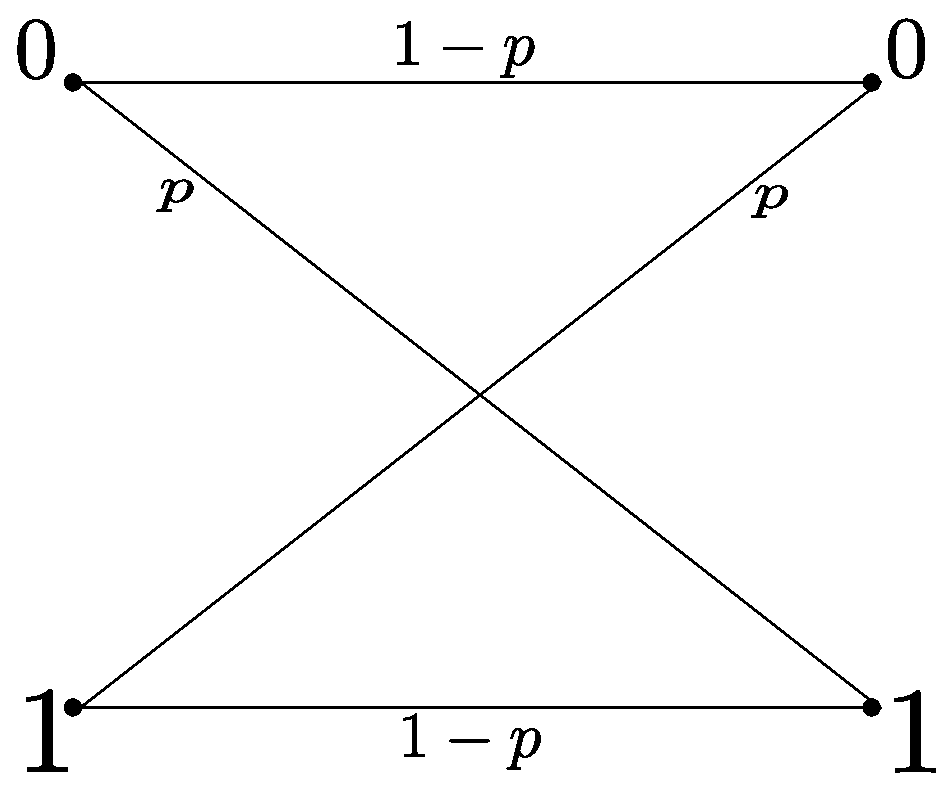
\includegraphics[scale=0.3]{Figures/Chapter2/dmc_3.eps}
                \caption{Input-Output graph of the BSC.}
                \label{fig_2.4}
            \end{figure}

        \item[(2)] If we take a DMC with $r=2$ and  $s=3$, then we have inputs
            $0$ and $1$, and outputs $0$, $1$, and $2$, where we take $2$ to be
            an  \textbf{erasure} of the input bit. We call this cahnnel a
            \textbf{binary erasure channel}. Such channels may arise if the
            inputs into such a (physical) channel were two sqare waves
            signifying voltage. Such waves are rarely perfect, and are often
            recieved in analog form with noise. Thus it is entriely possible for
            a bit going through this channel is erased.
    \end{enumerate}
\end{example}

\begin{lemma}\label{2.1.3}
    For any discrete memoryless channel, there is a pair of discrete random
    variables $X$ and $Y$ such that the channel takes $X \rightarrow Y$.
    Conversely, for any pair of discrete random variables, $(X,Y)$, there is a
    discrete memoryless channel taking $X \rightarrow Y$.
\end{lemma}
\begin{proof}
    Select the inputs, $X$, according to the probaility distribution  $p(x)$ on
     $\faktor{\Z}{r\Z}$. Now, define the random variable $Y$, then
     $p(x,y)=p(x)p(y|x)$, then $p y)=\sum_{x}{p(y|x)p(x)}$. We also get $p
     (x|y)=\frac{p(x,y)}{p(y)}$ which g ves us the result.
\end{proof}

\begin{example}
    \begin{enumerate}
        \item[(1)]
            \begin{figure}
                \centering
                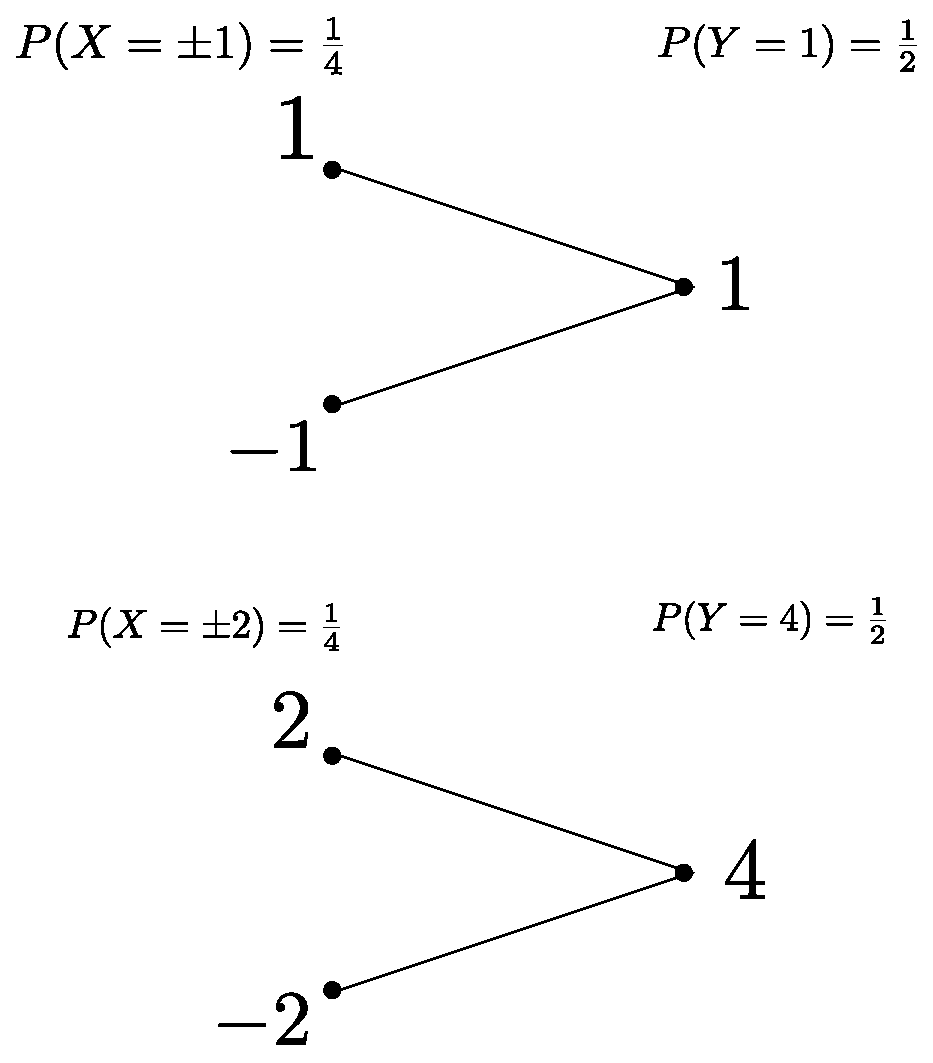
\includegraphics[scale=0.5]{Figures/Chapter2/dmc_4.eps}
                \caption{}
                \label{fing_2.5}
            \end{figure}
            Let $X$ be defined by the probabilities
            $P(X=1)=P(X=-1)=P(X=2)=P(X=-2)=\frac{1}{4}$ and $Y=X^2$. We get the DMC
            found in figure \ref {fig_2.5} from the pair $(X,X^2)$

        \item[(2)] Consider the Binary Erasure channeldescribed in example
            $2.3(2)$, where $2$ is the erasure of a single bit. We induce the
            DMC to be the graph: $0 \rightarrow 0$, $0 \rightarrow 2$, $1
            \rightarrow 2$, and $1 \rightarrow 1$ with the following
            probabilities: $\frac{3}{4}$, $\frac{1}{4}$, $\frac{1}{2}$, and
            $\frac{1}{2}$, respectively (see figure \ref{2.6}).
            \begin{figure}
                \centering
                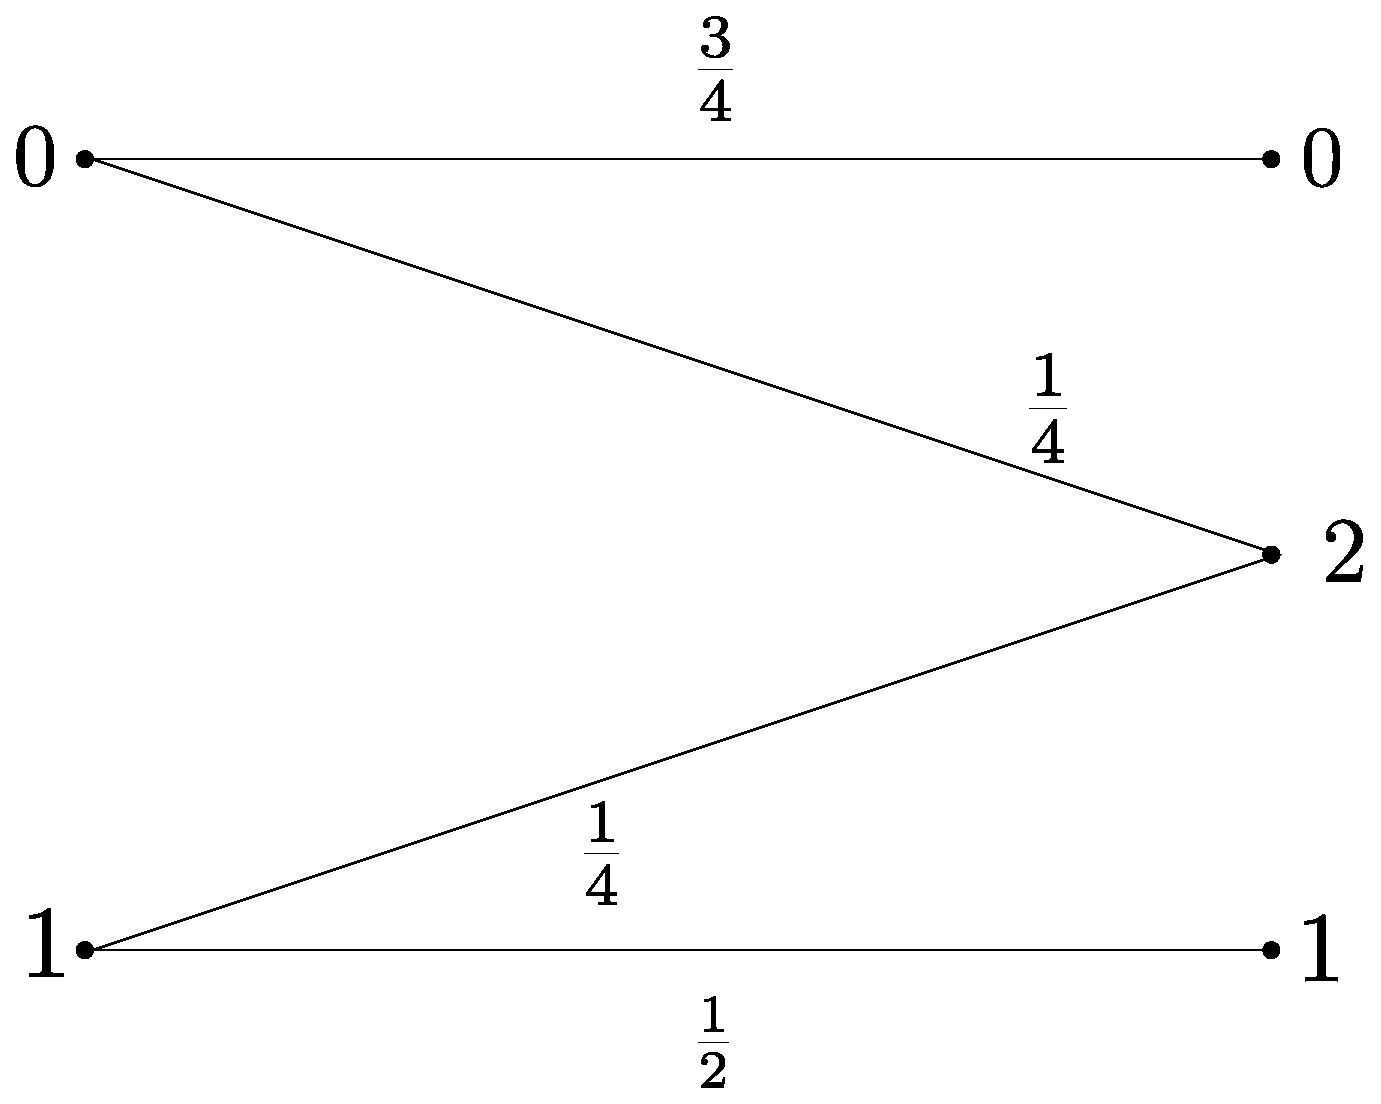
\includegraphics[scale=0.2]{Figures/Chapter2/bec_1.eps}
                \caption{}
                \label{fig_2.6}
            \end{figure}
            Let $P(X=0)=\frac{2}{3}$ and $P(X=1)=\frac{1}{3}$. Then we get
            $H(X)=\frac{2}{3}\log{\frac{3}{2}}+\frac{1}{3}\log{3}$ bits.
            Additionally, $H(X|Y=0)=0$, $H(X|Y=1)=0$ and $H(X|Y=2)=1$. So if $Y$
            is the erasure of a bit, there must be uncertainty about  $X$.
            Fortunately, on average we have certainty, so we can be confident
            the correct bit was transmitted.
    \end{enumerate}
\end{example}

\begin{theorem}\label{2.1.4}
    Let $X$,  $Y$, and  $Z$ be discrete random variables. Define for each  $z$,
     $A(z)=\sum_{x,y}{p(y)p(x|x,y)}$. Then:
     \begin{equation}
         H(X|Y) \leq H(Z)+E(\log{A})
     \end{equation}
\end{theorem}
\begin{proof}
    By definition,
     \begin{equation*}
        H(X|Y)=E(\log{\inv{p{x|y}}})=\sum_{x,y,z}{p(x,y,
        z)\log{\inv{p(x|y)}}}=\sum{p(z)}\sum\frac{p(x,y,z)}{p(z)}\log{\inv{p(x|y)}}
     \end{equation*}
    Now, fixing $z$ we get $\frac{p(x,y,z)}{p(z)}=p(x,y|z)$. Now, by Jensen's
    inequality to the inner sum, we get
    \begin{equation*}
        H(X|Y) \leq
        \sum{p(z)}\log{(\frac{1}{p(z)}\sum{\frac{p(x,y,
        z)}{p(x|y)}})}=\sum{p(z)\log{\inv{p(z)}}}+\sum{p(z)\log{\sum{\frac{p(x,y,
        z)}{p(x|y)}}}}
    \end{equation*}
    Now, $\frac{p(x,y,z)}{p(x|y)}=\frac{p(x,y,z)p(y)}{p(x,y)}=p(y)p(z|x,y)$ ;
    which establishes the result.
\end{proof}
\begin{corollary}[Fano's Inequality]
    If $X$ and $Y$ each take values in the sequence $\{x_i\}_{i=1}^r$, and
    $P_e=P(X \neq Y)$, then
    \begin{equation}
        H(X|Y) \leq H(P_e)+P_e\log{r-1}
    \end{equation}
\end{corollary}
\begin{proof}
    Take $Z=0$ if  $X=Y$ and  $Z=1$ if  $X \neq Y$. Then  $A(0)=1$ and
    $A(1)=r-1$.
\end{proof}

\begin{example}
    COnsider the DMC of example $2.4$. Taking  $r=3$,  $P(X=Y)=\frac{2}{3}$, and
    $P_e=\frac{1}{3}$, we get $H(X|Y) \leq
    H(\frac{1}{3})+\frac{1}{3}\log{2}=\frac{1}{3}\log{3}+\frac{2}{3}\log{\frac{3}{2}}+
    \frac{1}{3}\log{2}=\log{3}-\frac{1}{3}$ bits.
\end{example}

\begin{definition}
    Let $X$ and  $Y$ be random variables. Let $H(X)$ be the entropy of $X$
    independent of  $Y$, and $H(X|Y)$ the entropy of $X$ geven  $Y$. We define
    the  \textbf{mutual information} between $X$ and  $Y$ to be:
    \begin{equation}
        I(X,Y)=H(X)-H(X|Y)
    \end{equation}
    We define the \textbf{mutual information} of the random variables $X$,  $Y$,
    and  $Z$ to be:
    \begin{equation}
        I(X,Y,Z)=E(\log{\frac{p(z|x,y)}{p(z)}})
    \end{equation}
\end{definition}

\begin{lemma}\label{2.1.5}
    Given random variables $X$ and  $Y$, we have
    \begin{equation}
        I(X,Y)=\sum_{x,y}{p(x,y)\log{p(x|y)\inv{p(x)}}}=\sum{p(x,y)\log{\frac{p(x,
        y)}{p(x)p(y)}}}=\sum{p(x,y)\log{p(y|x)\inv{p(y)}}}
    \end{equation}
\end{lemma}
\begin{proof}
    $I(X,Y)=H(X)-H(X|Y)=\sum{p(x)\log{\inv{p(x)}}}-\sum{p(x,y)\log{\inv{p(x,y)}}}$.
\end{proof}

\begin{definition}
    We define the \textbf{joint entropy} between the random variables $X$ and
    $Y$ to be:
    \begin{equation}
        H(X,Y)=\sum{p(x,y)\log{\inv{p(x,y)}}}
    \end{equation}
\end{definition}

\begin{lemma}\label{2.1.6}
    The following hold:
    \begin{enumerate}
        \item[(1)] $I(X,Y)=I(Y,X)$.

        \item[(2)] $I(X,Y)=H(Y)-H(Y|X)$.

        \item[(3)] $I(X,Y)=H(X)+H(Y)-H(X,Y)$.
    \end{enumerate}
\end{lemma}
\begin{proof}
    By the above lemma, $I(X,Y)=\sum{p(x,y)\log{p(y|x)\inv{p(y)}}}=I(Y,X)$. Now,
    from this we get $I(X,Y)=I(Y,X)=H(Y)-H(Y|X)$, by definition.

    Now notice that $H(X,Y)=H(X)+H(Y|X)$. So $I(X,Y)=I(Y,X)=H(X)+H(Y)-H(Y|X)$.
\end{proof}

\begin{lemma}\label{2.1.7}
    For any discrete random variables $X$, and  $Y$,  $I(X,Y) \geq 0$. Moreover,
    $I(X,Y)=0$ if, and only if $X$ and  $Y$ are independent of each other.
\end{lemma}
\begin{proof}
    That $I(X,Y) \geq 0$ follows from definition. Now, if $I(X,Y)=0$, then
    $H(X)+H(Y)=H(X,Y)$ which implies independence. Conversely, we get that same
    result.
\end{proof}

\begin{theorem}\label{2.1.8}
    Given discrete random variables $X$,  $Y$, and  $Z$,  $I(X,Y,Z) \geq
    I(Y,Z)$, with equality holding if, and only if $p(z|x,y)=p(z|y)$ for all
    triples $(x,y,z)$ and $p(x,y,z)>0$.
\end{theorem}
\begin{proof}
    $I(Y,Z)-I(X,Y,Z)=E(\log{\frac{p(z|y)}{p(z)}}-\log{\frac{p(z|x,y)}{p(z)}})=
    E(\log{\frac{p(z|y)}{p(z|x,y)}})=\sum{p(x,y,z)\log{\frac{p(x|y)}{p(z|x,y)}}}$.
    Now, by Jensen's inequality, $I(Y,Z)-I(X,Y,Z) \leq \log{\sum{p(x,y,
    z)\frac{p(x|y)}{p(z|x,y)}}}=\log{1}=0$.
\end{proof}

We can state the above results in terms of Markov chains.

\begin{theorem}\label{2.1.9}
    If $(X,Y,Z)$ is a Markov chain, then
    \begin{equation}
        I(X,Z)=\begin{cases}
                    I(X,Z)  \\
                    I(Y,Z)  \\
               \end{cases}
    \end{equation}
\end{theorem}

\begin{example}
    \begin{enumerate}
        \item[(1)]If $X_1,X_2,X_3$ are independent random variables, then the triple
        $(X_1,X_1+X_1,X_1+X_2+X_3)$ forms a Markov chain. So $I(X_1,X_1+X_2+X_3)
        \leq I(X_1,X_1+X_2)$.

    \item[(2)] Define $X$ by  $P(X=0)=P(X=1)=\frac{1}{2}$, on two DMCs both
        with error proabilities  $p$. Then  $I(X,Y)=1-H(p)$ and
        $I(X,Z)=1-H(2p(1-p))$.
    \end{enumerate}
\end{example}

\begin{theorem}\label{2.1.10}
    Given discrete random variables $X$ and  $Y$, $I(X,Y)$ is a convex down
    function of the probabilities $p(x)$.
\end{theorem}
\begin{proof}
    Fix the transformation probabilities $p(y|x)$, and let $X_1$ and $X_2$ be
    two random variables with probability distributions $p_1(x)$ and $p_2(x)$.
    Define the probability distribution of $X$ to be the convex combination
    $p(x)=\alpha p_1(x)_\beta p_2(x)$.

    Now, consider $Y_1,Y_1$, and $Y$ such that  $X_1 \rightarrow Y_1$, $X_2
    \rightarrow Y_2$, and $X \rightarrow Y$ through some DMC. Then we must have:
    \begin{equation*}
        \alpha I(X_1,Y_1)+\beta
        I(X_2,Y_2)-I(X,Y)=\sum{p_1(x)\log{\frac{p(y)}{p_1(y)}}}+
        \sum{p_2(x)\log{\frac{p(y)}{p_2(y)}}}
    \end{equation*}
    By Jensen's inequality, we get:
    \begin{equation*}
        \sum{p_1(x)\log{\frac{p(y)}{p_1(y)}}} &\leq \log{\sum{p_1(x,
        y)\frac{p(y)}{p_1(y)}}}=\log{\sum{\frac{p(y)}{p_1(y)}p_1(y)}}=1
    \end{equation*}
    Hence, both sums are less than $0$, which makes  $I(X,Y)$ convex down.
\end{proof}
\begin{corollary}
    The entropy of the proabilitie vector $p=(p_1, \dots, p_r)$, $H(p)$ is
    convex down.
\end{corollary}
\begin{proof}
    Define $X$ by the distribution  $P(X=x_i)=p_i$. Then $I(X,X)=H(X)=H(p)$
    where $p=(p_1, \dots, p_r)$.
\end{proof}

\begin{theorem}\label{2.1.11}
    $I(X,Y)$ is convex up in the transition probabilities $p(y|x)$.
\end{theorem}
\begin{proof}
    The proof is analogous to that of theorem \ref{2.1.10}.
\end{proof}
